\clearpage\nobalance
\section*{Author Notes}
\subsection*{Acknowledgements}
I thank Prof. Luyao Zhang, Program Chair, and Prof. Ken Rogerson, Program Discussant, of the \emph{2056 Nobel and Turing Laureate Program Launch Workshop}, held at Duke Kunshan University on September 7, 2026. I participated in Session B, ``When Does an LLM Promise Become Trustworthy?,'' as Speaker 2 for Computer Science. Muhan Chen's economics framing of incentives and reputation helped sharpen the idea that historical reliability is an allocation signal whose use can change who receives access to scarce attention. Xinrong Sun's behavioral framing of trust helped motivate the distinction between interruption burden and trust loss. Their contributions supplied interdisciplinary workshop context; neither is a coauthor or designer of the interruption-authority model. I, Yiqiao Liu, am responsible for the proposal and remaining errors.

\subsection*{Individual contribution}
I selected the research direction and formulated the central question of interruption authority among specialized AI agents. I chose the 20-minute research-brief scenario; the Evidence, Planning, and Idea roles; the current importance-and-urgency plus task-specific historical-reliability framing; and the evaluation questions concerning attention, missed warnings, unequal voice, burden, trust, and oversight. I reviewed and approved the model assumptions, interpreted the synthetic results, checked Git diffs and saved outputs, personally performed the fresh Google Colab Run All check, personally checked the deployed Hugging Face Space, and verified the final citations and evidence boundaries. ChatGPT and Codex assisted with implementation, testing, figures, notebook and demo construction, drafting, debugging, and compilation, as detailed in Appendix A.1; I do not claim to have manually authored every line of code.

\bibliographystyle{ACM-Reference-Format}\bibliography{references}
\appendix
\section{Technical details and reproducibility}
\paragraph{Model and routing.}
For normalized importance $I$ and urgency $U$, the current-claim score is
\[
N=0.5I+0.5U.
\]
The current-claim policy uses $S=N$; the proposed reputation-calibrated policy uses $S=NR$. Task-specific historical reliability applies Beta$(1,1)$ smoothing,
\[
R=\frac{\text{valid}+1}{\text{audited}+2}.
\]
The authored histories are Evidence $17/18$ ($R=0.90$), Planning $9/18$ ($R=0.50$), and Idea $3/18$ ($R=0.20$); an unseen agent--task pair receives the cold-start value $R=0.50$. A score $S\geq0.65$ interrupts immediately, $0.35\leq S<0.65$ queues, and $S<0.35$ enters the minute-20 digest. A queued report goes to the strictly next five-minute checkpoint: arrivals at minutes 4, 5, 9, and 10 deliver at 5, 10, 10, and 15, respectively. The session horizon is 20 minutes.

\paragraph{Inputs and evidence boundary.}
The fixed diagnostic contains exactly 18 authored deterministic synthetic notifications: six each from Evidence, Planning, and Idea. The report records contain only claims visible to an online policy. Validity, late-loss, and latest-useful-minute labels are stored separately and enter evaluation only after routing; hidden outcomes never enter the online scheduling rule. The files are not participant data, real LLM outputs, field observations, deployment evidence, or safety validation. No random seed is required because both data and scheduling are deterministic.

\paragraph{Metrics.}
An important alert is a report with \texttt{valid} equal to true and \texttt{late\_loss} at least 7. Per-message attention costs are 2.0 for interrupt, 0.2 for queue, and 0.05 for digest. Synthetic joint loss is attention cost plus late-alert loss. Evaluation also audits interruption count, invalid interruptions, timely recall, and per-agent routing and authority.

\paragraph{Verified online results.}
\begin{center}
\small
\begin{tabular}{@{}lrr@{}}
\toprule
\textbf{Metric} & \textbf{Current claim} & \textbf{Reputation} \\
\midrule
Interrupt / queue / digest & 10 / 5 / 3 & 2 / 4 / 12 \\
Invalid immediate notices & 4 & 1 \\
Invalid interruption fraction & 0.40 & 0.50 \\
Important alerts timely & 8 / 8 & 2 / 8 \\
Timely recall & 1.00 & 0.25 \\
Attention cost & 21.15 & 5.40 \\
Late-alert loss & 0.00 & 49.00 \\
Synthetic joint loss & 21.15 & 54.40 \\
\bottomrule
\end{tabular}
\end{center}
The multiplicative rule saves attention in this authored scenario but performs worse on important-alert timely recall and synthetic joint loss; it is not superior. Swapping the Evidence and Idea histories gives reputation-calibrated routing of 3 interrupts, 3 queues, and 12 digests, timely recall 0.125, and joint loss 66.20.

\paragraph{Equal-count offline ranking diagnostic.}
Each ranking receives ten immediate slots; all eight non-selected reports use the identical next-checkpoint queue fallback, and no digest route appears. Both rankings therefore have 10 interrupts, 8 queues, timely recall 1.00, attention cost 21.60, and joint loss 21.60. Current-claim slots are Evidence 3, Planning 3, and Idea 4; reputation-ranking slots are Evidence 6, Planning 4, and Idea 0. This offline diagnostic isolates authority allocation under a fixed interruption budget; it is not an online deployment policy.

\begingroup
\raggedright
\paragraph{Reproducibility record.}
The Python implementation is \path{companion/src/}\path{scheduler.py}. The inputs in \path{companion/data/} are \path{reports.json}, \path{history.json}, and \path{outcomes.json}. The project-specific tests are in \path{companion/tests/}\path{test_scheduler.py}, and the experiment runner is \path{companion/scripts/}\path{run_experiment.py}. Saved outputs under \path{companion/outputs/} are \path{interruption_authority_results.json} and \path{interruption_authority_decisions.csv}. The executable notebook is \path{companion/notebooks/}\path{PS1_attention.ipynb}, and the demo source is under \path{companion/hf_space/}. Public repository, notebook, and hosted-demo links appear in the main paper.

The computational core, notebook, and interactive demo were checkpointed at \texttt{343fb3e}, \texttt{f3a1065}, and \texttt{9c5cb05}; this supporting-material revision began from \texttt{dc57ab3}, not from a self-referential release hash. On Python 3.13.5, all 18 project-specific scheduler tests passed. Yiqiao Liu manually verified a fresh Colab Run All execution and the hosted Hugging Face demo.
\par
\endgroup

\subsection{AI-use disclosure}
Tools used were ChatGPT and Codex, primarily on September 12--13, 2026. The ChatGPT working interface identified GPT-5.6 Sol; the exact underlying Codex model snapshot was not exposed and is not guessed here. I, Yiqiao Liu, independently selected the research direction, multi-agent interruption authority as the main problem, the use of current importance and urgency with task-specific historical reliability, the 20-minute research-brief scenario, the three specialized agent roles, and the focus on oversight, attention, missed warnings, unequal voice, burden, and trust.

AI assistance was more substantial than grammar polishing. It helped formalize the $N$ and $S$ heuristics; structure the five-section paper; construct and refine authored synthetic diagnostic cases; implement Python code and unit tests; debug equal-count and history-swap diagnostics; construct the notebook, Hugging Face interface, and editable figure; draft and revise explanatory prose; compile and paginate LaTeX; and guide GitHub, Colab, and Hugging Face workflows. A concrete human-verified correction changed the equal-count diagnostic so every non-selected report uses the same queue fallback, preventing queue-versus-digest score shrinkage from being mistaken for ranking quality. Suggestions implying superiority, optimality, empirical validation, or naturally occurring data were rejected or qualified.

I reviewed diffs, tests, and outputs; ran and verified the fresh Colab execution; verified the hosted demo, citations, and evidence boundaries; and decided which AI suggestions to accept. The synthetic cases are authored diagnostics created and refined with AI implementation assistance, not naturally occurring data. I remain responsible for assumptions, interpretation, citations, verification, and submission. AI did not originate the research direction.

\section{Cumulative Intellectual Development}
The inquiry began with the broad ACT/DEFER question: when should an AI system act autonomously, and when should it defer to a human? I narrowed it to multi-agent interruption authority: when specialized agents compete for limited human attention, who gets to interrupt? I then added task-specific historical reliability to current importance and urgency as a possible allocation signal.

The deterministic diagnostic changed the intellectual emphasis. Naively multiplying by reliability sharply reduced interruptions, but it also delayed important warnings and concentrated authority. The guiding question therefore shifted from ``Can reputation reduce unnecessary interruption?'' to ``How much should history affect interruption rights without creating missed warnings, unequal voice, or self-reinforcing silence?'' Economics frames scarce attention, allocation, costs, and incentives; computer science supplies a transparent, auditable, reproducible scheduler; and behavioral science separates interruption burden from trust loss.

This development was situated in the September 7, 2026 workshop at Duke Kunshan University, Session B---``When Does an LLM Promise Become Trustworthy?''---where I served as Speaker 2 for Computer Science with teammates Muhan Chen and Xinrong Sun. Muhan's economics framing of incentives and reputation sharpened the allocation-signal interpretation; Xinrong's behavioral framing of trust motivated the burden-versus-trust distinction. These were interdisciplinary inputs, not coauthorship or design of the interruption-authority model. Appendix~\ref{app:abstract} records the V1 structured abstract.

\section{Field and open-source inspiration}
I participated in the September 4, 2026 \emph{Joint Interdisciplinary Field Trip---Technology, Computation, Culture \& Society in Action}, including work at Tencent Shanghai Office and Shanghai Science and Technology Museum.

\begin{figure}[H]
\centering

\includegraphics[height=0.28\textheight,angle=270,origin=c]{figures/field_tencent.jpg}
\caption{Tencent Shanghai Office, September 4, 2026. The visible exhibit sign identifies ``5G AV Remote Control Industrial vehicles.'' The display motivated attention to explicit control handoff, escalation, and accountable human oversight rather than assuming that greater autonomy is always preferable. Source: Yiqiao Liu's Week 2 field-trip course materials. This observation motivates the research question but does not validate the scheduler.}
\Description{Portrait field-trip photograph of a Tencent Shanghai Office exhibit. A curved illuminated sign reads 5G AV Remote Control Industrial vehicles above a dark technology display.}
\label{fig:field-tencent}
\end{figure}

\begin{figure}[H]
\centering
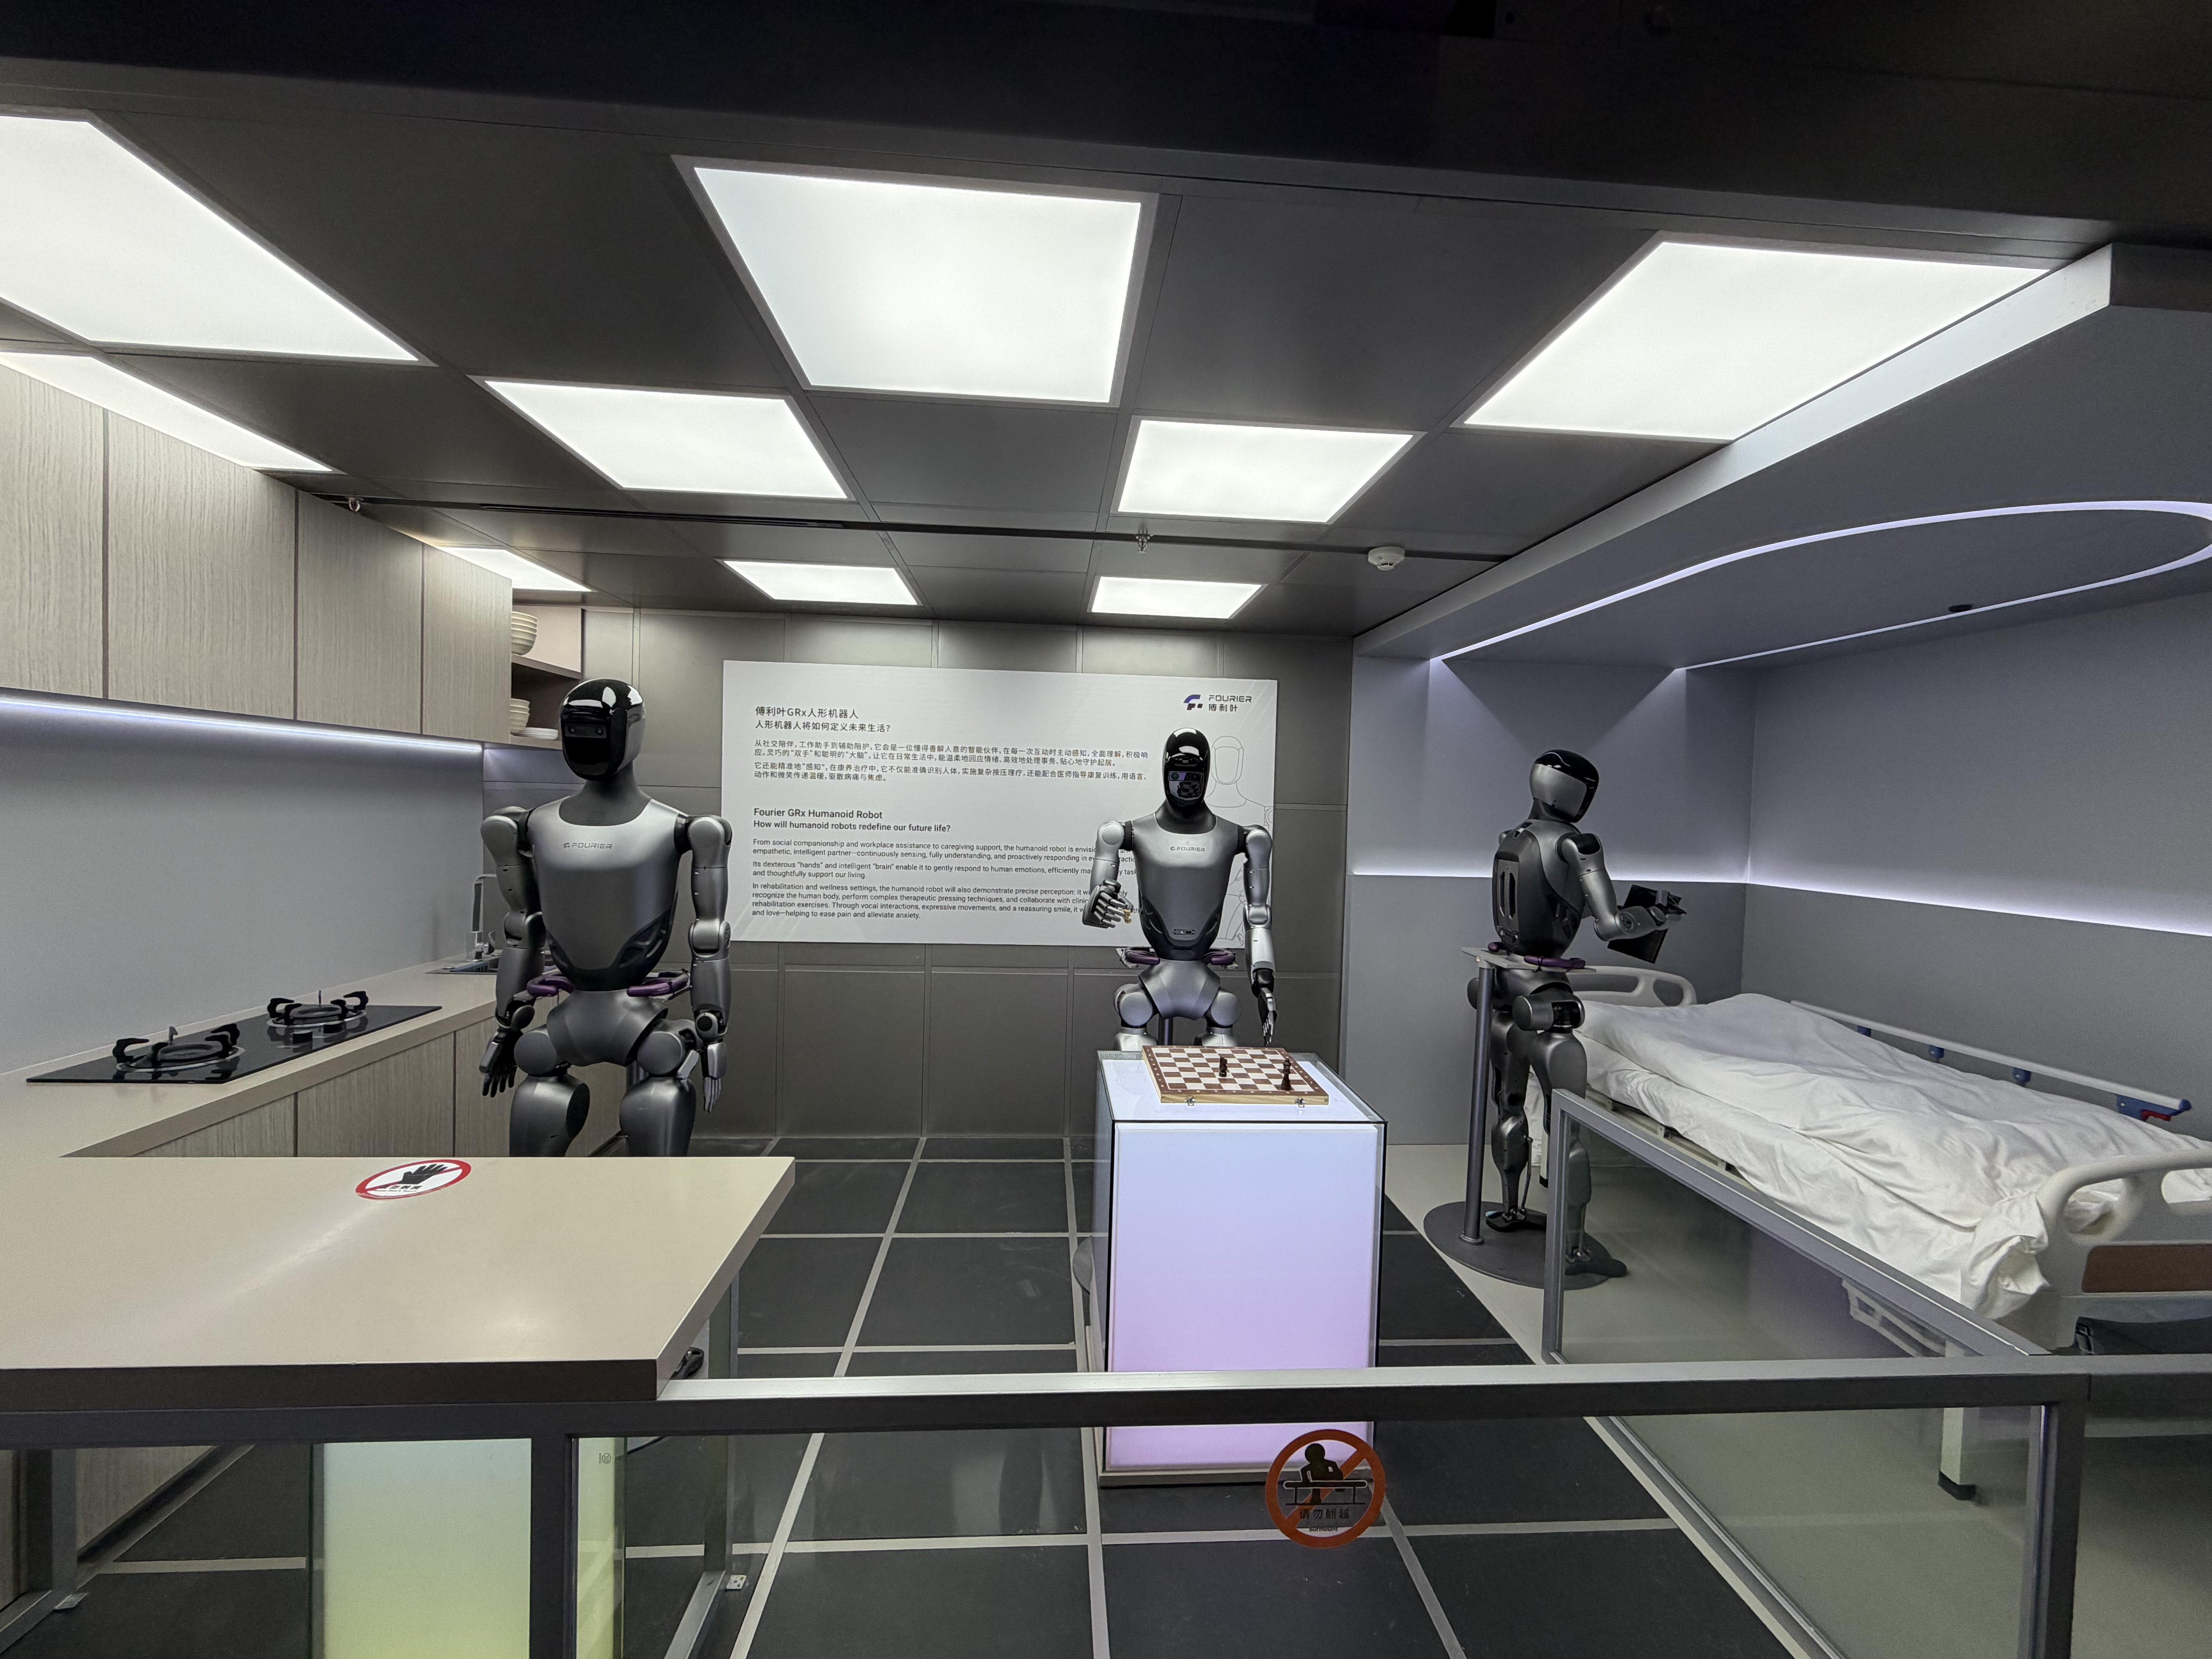
\includegraphics[width=\columnwidth]{figures/field_museum.jpg}
\caption{Shanghai Science and Technology Museum, September 4, 2026. Three humanoid robots are visibly staged in a domestic and caregiving display with kitchen, game-table, and bedside settings. The varied public-facing contexts motivate context-sensitive consequences for autonomy, oversight, and interruption authority. Source: Yiqiao Liu's Week 2 field-trip course materials. This observation motivates the research question but does not validate the scheduler.}
\Description{Landscape field-trip photograph of three humanoid robots staged in an exhibit with kitchen counters, a game table, and a hospital-style bed.}
\label{fig:field-museum}
\end{figure}

The project's transparent routing logic, public GitHub code, reproducible Colab notebook, and open interactive Hugging Face demonstration are an open-source response intended to make oversight mechanisms inspectable. They operationalize the research question for audit and discussion; neither the artifacts nor the field observations constitute empirical validation.

\newpage
\section{Review response and revision record}
This is V1, dated September 13, 2026. Human-Only peer review is scheduled for September 14, 2026; no peer review, rebuttal, reviewer follow-up, or V2 exists yet. Later versions will append those records rather than overwrite V1.

Before review, the broad ACT/DEFER question was narrowed to interruption authority; a project-specific Figure 1 replaced the template figure; the computational core was implemented and tested; and the Colab notebook and Hugging Face artifact were verified. The equal-count diagnostic was corrected so non-selected reports receive identical queue fallback treatment. The interpretation was also revised to state explicitly that naive multiplicative reputation performs worse in the authored online diagnostic. These are pre-review development records, not peer-review revisions.

\clearpage\onecolumn
\section{Structured abstract and cumulative proposal map}\label{app:abstract}
\begin{table}[H]
\caption{V1 structured abstract and cumulative proposal map.}
\label{tab:abstract-map}
\small
\renewcommand{\arraystretch}{1.10}
\begin{tabularx}{\textwidth}{@{}p{0.24\textwidth}Y@{}}
\toprule
\textbf{Proposal element} & \textbf{Current statement / change} \\
\midrule
Background & Multiple specialized AI agents can compete for scarce human attention. Nash and Harsanyi supply strategic and incomplete-information lineage; Newell and Simon connect AI, cognition, bounded rationality, and organizational authority~\cite{nash1950,harsanyi1968,nobel1994game,acm1975newellsimon,simon1978lecture}. The unresolved issue is how modern AI agents should earn interruption authority. \\
Motivation and application & In a 20-minute research brief, Evidence, Planning, and Idea Agents submit candidate messages. False interruptions consume attention, while delayed valid warnings can be costly. Users, agent designers, and organizations need an inspectable allocation rule. \\
Three connected questions & \textbf{Economics:} When does historical reliability improve scarce-attention allocation, and who bears interruption and missed-warning costs? \textbf{Computation:} Can a transparent history-calibrated scheduler reduce unnecessary interruptions without delaying too many important messages? \textbf{Behavior:} Is lower response caused by cognitive burden or trust loss after false alarms? \textbf{Integrated:} How should current claims and task-specific history determine interrupt, queue, or digest while preserving human oversight? \\
Method and model assumptions & $N=0.5I+0.5U$; baseline $S=N$; proposed $S=NR$; Beta-smoothed task-specific $R$; shared thresholds; 18 authored deterministic synthetic notifications; and evaluation-only hidden outcomes. Diagnostics compare current-claim, history-calibrated, history-swap, and equal-count rules. \\
Results or expected results & \textbf{Synthetic result:} current-claim joint loss is 21.15 with timely recall 1.00; multiplicative-reputation joint loss is 54.40 with timely recall 0.25. At equal count, joint loss is 21.60 for both, but Idea's immediate authority falls from four slots to zero. Future human and real-agent studies should test burden, trust, domain shift, reputation recovery, and strategic reporting. \\
Intellectual merits & The contribution is not mathematical novelty of multiplication. It is a falsifiable, inspectable allocation question connecting historical validity to the right to interrupt, with audits of saved attention, missed warnings, and unequal voice across economics, computer science, and behavioral science. \\
Practical impacts & The framework may inform multi-agent assistants, notification systems, and human oversight. Public GitHub, Colab, and Hugging Face artifacts make the mechanism inspectable. The learning tool is relevant to SDG 4, but no measured educational benefit is claimed. \\
Feedback received and revision made & This is V1 before formal Human-Only peer review, scheduled for September 14, 2026. Pre-review development moved from ACT/DEFER to interruption authority, added historical reliability, and used diagnostic evidence to expose missed-warning and unequal-authority risks. The equal-count diagnostic was corrected so fallback treatment is identical. No reviewer comment is claimed. \\
\bottomrule
\end{tabularx}
\end{table}
